\documentclass[crop,tikz]{standalone}% 'crop' is the default for v1.0, before it was 'preview'
%\usetikzlibrary{...}% tikz package already loaded by 'tikz' option
\begin{document}
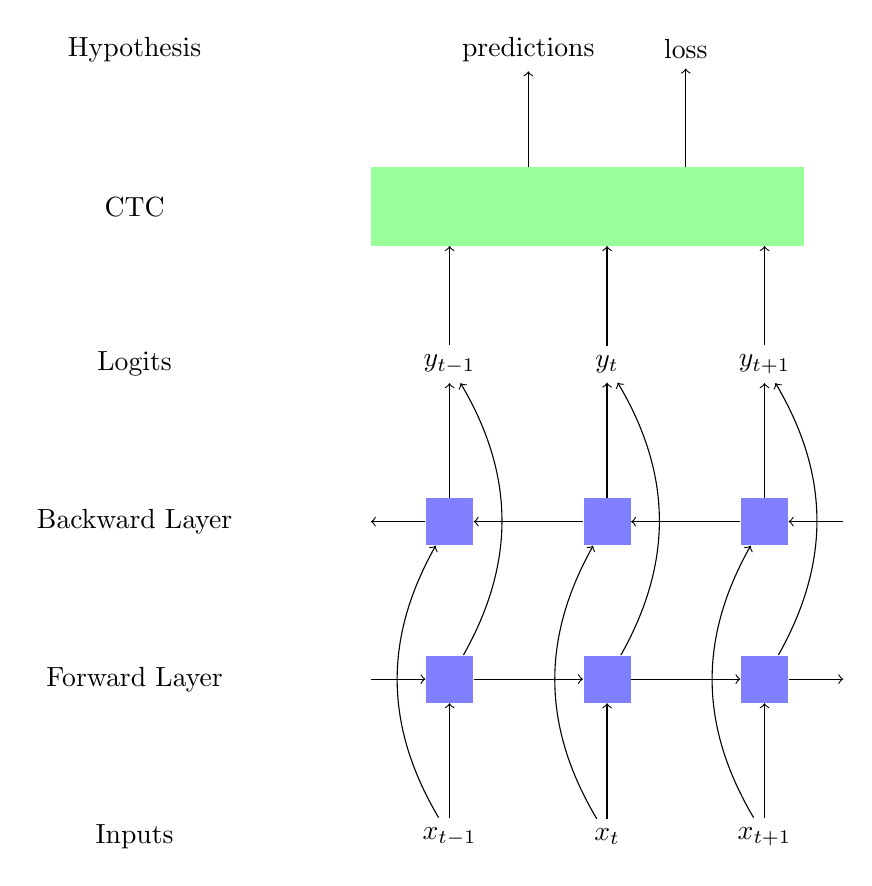
\begin{tikzpicture}
\tikzstyle{rcNeuron}=[rectangle,fill=black!25,minimum size=17pt,inner sep=0pt]
\tikzstyle{LSTM}=[rcNeuron, fill=blue!50];
%Layer Marks
\node (hypothesis)    at (0,10){Hypothesis};
\node (CTC)   		  at (0,8) {CTC};
\node (outputLabel)   at (0,6) {Logits};
\node (backwardLabel) at (0,4) {Backward Layer};
\node (forwardLabel)  at (0,2) {Forward Layer};
\node (inputLabel)    at (0,0) {Inputs};

%input nodes.
\node (xtm1) at (4,0) {$x_{t-1}$};
\node (xt)   at (6,0) {$x_{t}$};
\node (xtp1) at (8,0) {$x_{t+1}$};

%output nodes
\node (ytm1) at (4,6) {$y_{t-1}$};
\node (yt)   at (6,6) {$y_{t}$};
\node (ytp1) at (8,6) {$y_{t+1}$};

% forward lstm blocks.
\node[LSTM] (forwardXtm1) at (4,2) {};
\node[LSTM] (forwardXt) at (6,2) {};
\node[LSTM] (forwardXtp1) at (8,2) {};

% backward lstm blocks.
\node[LSTM] (backwardXtm1) at (4,4) {};
\node[LSTM] (backwardXt) at (6,4) {};
\node[LSTM] (backwardXtp1) at (8,4) {};

%CTC layer
\fill[green!40!white] (3,7.5) rectangle (8.5,8.5);

% connections
\draw[->] (3,2)         -- (forwardXtm1);
\draw[->] (forwardXtm1) -- (forwardXt);
\draw[->] (forwardXt)   -- (forwardXtp1);
\draw[->] (forwardXtp1) -- (9,2);

\draw[->] (backwardXtm1) -- (3,4);
\draw[->] (backwardXt) -- (backwardXtm1);
\draw[->] (backwardXtp1) -- (backwardXt);
\draw[->] (9,4) -- (backwardXtp1);

\draw[->] (xtm1) -- (forwardXtm1);
\draw[->] (xt) -- (forwardXt);
\draw[->] (xtp1) -- (forwardXtp1);

\draw[->, bend angle=30, bend left] (xtm1) to (backwardXtm1);
\draw[->, bend angle=30, bend left] (xt) to (backwardXt);
\draw[->, bend angle=30, bend left] (xtp1) to (backwardXtp1);

\draw[->, bend angle=30, bend right] (forwardXtm1) to (ytm1);
\draw[->, bend angle=30, bend right] (forwardXt) to (yt);
\draw[->, bend angle=30, bend right] (forwardXtp1) to (ytp1);

\draw[->] (backwardXtm1) -- (ytm1);
\draw[->] (backwardXt) -- (yt);
\draw[->] (backwardXtp1) -- (ytp1);

%CTC connections
\draw[->] (ytm1) -- (4,7.5);
\draw[->] (yt)   -- (6,7.5);
\draw[->] (ytp1) -- (8,7.5);

\node (pred) at (5,10) {predictions};
\node (loss) at (7,10) {loss};

\draw[->] (5,8.5) -- (pred);
\draw[->] (7,8.5) -- (loss);

\end{tikzpicture}
\end{document}